% Suggested LaTeX style template for Masters project report submitted at the
% Department of Computer Science and Technology
%
% Markus Kuhn, May 2022
% (borrowing elements from an earlier template by Steven Hand)

\documentclass[12pt,a4paper,twoside]{report}
% append option ",openright" after "twoside" if you prefer each chapter
% to start on a recto (odd-numbered) page in a double-sided printout

\usepackage[pdfborder={0 0 0}]{hyperref}
\usepackage[vmargin=20mm,hmargin=25mm]{geometry}
\usepackage{graphicx}
\usepackage{parskip}
\usepackage{setspace}
\usepackage{refcount}
\usepackage{upquote}
\usepackage{xcolor}
\usepackage{subcaption}
\usepackage{amsmath}
\usepackage{amssymb}
\usepackage[sort,numbers]{natbib}
\usepackage[capitalise]{cleveref}
\usepackage{adjustbox}
\usepackage{listings}
\usepackage{float}
\usepackage{tabularx}
\usepackage{booktabs}
\usepackage{multirow}
\usepackage{xspace}
\usepackage{tikz}
\usepackage{wrapfig}
\usepackage{nicefrac}
\usepackage{enumitem}
\usepackage{bbm}
\usepackage{pdflscape}

\usetikzlibrary{arrows,calc,arrows.meta,positioning}
\setlist[enumerate]{itemsep=1pt}
\lstset{
basicstyle=\small\ttfamily,
columns=fullflexible,
breaklines=true,
}
\hypersetup{
    colorlinks,
    linkcolor={blue!50!black},
    citecolor={blue!50!black},
    urlcolor={black}
}

\newif\ifsubmission % Boolean flag for distinguishing submitted/final version

% Change the following lines to your own project title, name, college, course
\title{End-to-End Ontology Learning with Large Language Models}
\author{Chun Yuen Andy Lo}
\date{May 2024}
\newcommand{\candidatenumber}{1234N}
\newcommand{\college}{Christ's College}
\newcommand{\course}{Computer Science Tripos, Part III}
\newcommand{\todo}[1]{\textcolor{red}{TODO: #1}}
\newcommand{\name}{{OLLM}\xspace}
\newcommand{\m}[1]{\mathbf{#1}}
\newcommand{\R}{\mathbb{R}}
\renewcommand{\O}{\mathcal{O}}
\newcommand{\E}{\mathcal{E}}
\newcommand{\V}{\mathcal{V}}
\newcommand{\D}{\mathcal{D}}
\DeclareMathOperator{\nodesim}{NodeSim}
\DeclareMathOperator{\cossim}{CosSim}
\DeclareMathOperator{\match}{match}

\hyphenpenalty=0

% Select which version this is:
% For the (anonymous) submission (without your name or acknowledgements)
% uncomment the following line (or let the makefile do this for you)
% \submissiontrue
% For the final version (with your name) leave the above commented.

\begin{document}

%TC:ignore 
\begin{sffamily} % use a sans-serif font for the pro-forma cover sheet

    \begin{titlepage}
        \makeatletter

        % University logo with shield hanging in left margin
        \hspace*{-14mm}
\includegraphics[width=65mm]{logo-dcst-colour.pdf}

        \ifsubmission

            % submission proforma cover page for blind marking
            \begin{Large}
                \vspace{20mm}
                Research project report title page

                \vspace{35mm}
                Candidate \candidatenumber

                \vspace{42mm}
                \textsl{``\@title''}

            \end{Large}

        \else

            % regular cover page
            \begin{center}
                \Huge
                \vspace{\fill}

                \@title
                \vspace{\fill}

                \@author
                \vspace{10mm}

                \Large
                \college
                \vspace{\fill}

                \@date
                \vspace{\fill}

            \end{center}

        \fi

        \vspace{\fill}
        \begin{center}
            Submitted in partial fulfillment of the requirements for the\\
            \course
        \end{center}

        \makeatother
    \end{titlepage}

    \newpage

    Total page count: \pageref{lastpage}

    % calculate number of pages from
    % \label{firstcontentpage} to \label{lastcontentpage} inclusive
    \makeatletter
    \@tempcnta=\getpagerefnumber{lastcontentpage}\relax%
    \advance\@tempcnta by -\getpagerefnumber{firstcontentpage}%
    \advance\@tempcnta by 1%
    \xdef\contentpages{\the\@tempcnta}%
    \makeatother

    Main chapters (excluding front-matter, references and appendix):
    \contentpages~pages
    (pp~\pageref{firstcontentpage}--\pageref{lastcontentpage})

    Main chapters word count: 10000\footnote{Computed with \texttt{texcount}.}

\end{sffamily}

\vspace{\fill}
\onehalfspacing
\makeatletter
\textbf{\Huge Declaration}
\vspace{40pt}

\ifsubmission
    I, [Blind candidate number], being a candidate for Part III of the Computer Science Tripos, hereby declare that this project report and the work described in it are my own work, unaided except as may be specified below, and that the project report does not contain material that has already been used to any substantial extent for a comparable purpose. The project required the use of AI-assisted platform GitHub Copilot in chapter 3 and 4, and such use is acknowledged in the text. I am content for my project report to be made available to the students and staff of the University.

    \bigskip
    \textbf{Date:} \today
\else
    I, \@author\ of \college, being a candidate for Part III of the Computer Science Tripos, hereby declare that this project report and the work described in it are my own work, unaided except as may be specified below, and that the project report does not contain material that has already been used to any substantial extent for a comparable purpose. The project required the use of AI-assisted platform GitHub Copilot in chapter 3 and 4, and such use is acknowledged in the text. I am content for my project report to be made available to the students and staff of the University.

    \bigskip
    \textbf{Signed:} \@author

    \bigskip
    \textbf{Date:} \today
\fi
\vspace{\fill}
\makeatother

\chapter*{Abstract}

Ontologies are useful for automatic machine processing as they represent knowledge in a structured format. Yet, constructing ontologies requires substantial manual effort. To automate part of this process, large language models (LLMs) have been applied to solve various subtasks of ontology learning. However, this partial ontology learning does not capture the interactions between subtasks.
We address this gap by introducing \name, a general and scalable method for solving the \emph{full} task of building an ontology from scratch.
Rather than focusing on subtasks, like individual relations between entities, we model entire subcomponents of the target ontology by finetuning an LLM with a custom regulariser that reduces overfitting on high-frequency concepts. We introduce a novel suite of metrics for evaluating the quality of the generated ontology by measuring its semantic and structural similarity to the ground truth. Our metrics stem from modern deep learning evaluation techniques, but make fewer assumptions about the ontologies than standard ontology metrics.
Our results on Wikipedia show that \name outperforms subtask composition methods, producing more semantically accurate ontologies while maintaining structural integrity. We further demonstrate that our model can be effectively adapted to a new domain, like arXiv, needing only a small number of training examples.

\ifsubmission\else
    % not included in submission for blind marking:

    \chapter*{Acknowledgements}

    This project would not have been possible without the wonderful
    support of \ldots [optional]

\fi
\cleardoublepage % preserve page numbers after missing acknowledgements

\tableofcontents
%\listoffigures
%\listoftables
%TC:endignore 

\chapter{Introduction}

\label{firstcontentpage} % start page count here

An ontology is a formal and structural way of representing domain-specific concepts and their relations~\cite{gruber1995toward}.
They can be simplistic consisting of \emph{concepts} and only a small number of types of \emph{taxonomic relations} (e.g., \emph{is-a} relationships). Or they can be complex consisting of axioms and many types of relations. For example, a simple ontology for programming languages might be:
\begin{figure}[H]
    \centering
    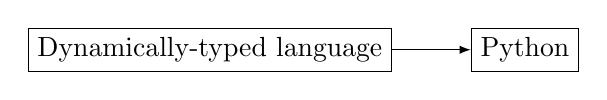
\begin{tikzpicture}[>=latex]
        \node[rectangle, draw] (dynamically-typed) {Dynamically-typed language};
        \node[rectangle, draw, right=of dynamically-typed] (python) {Python};
        \draw[->] (dynamically-typed) -- (python);
    \end{tikzpicture}
\end{figure}
\vspace{-1em}
It has two concepts and one relation, representing the knowledge that Python is a dynam\-ically-typed language. A more complex ontology might contain axioms too, for example, ``all programming languages are either dynamically or statically typed''. In this project, I focus on ontologies with only concepts and taxonomic relations. Compared to typical deep learning models which represent knowledge implicitly in its weights, ontologies capture knowledge in a structured and explicit manner, making them reliable, easy to edit and human-interpretable. Such benefits of ontologies have led to their wide adoption in practice. For example, the Wikipedia categories have been used for entity ranking~\cite{vercoustre2008using} and information retrieval~\cite{sorg2012exploiting} or the Schema.org~\cite{Schema.org_2011} ontology which is part of the Semantic Web~\cite{antoniou2004semantic} initiative.

While ontologies are useful, building ontologies often requires substantial manual effort. Ontology learning (OL) is the study of automating the construction of high-quality ontologies at scale. For a simplistic ontology, this amounts to discovering the concepts and taxonomic relations, usually based on a source corpus. This project aims contribute to this field by researching domain-independent methods for OL that are scalable and produce better ontologies.

\section{Project goals}

Traditionally, OL is viewed as a composition of subtasks~\cite{asim2018survey}, such as concept discovery and relation extraction. In particular, prior works have demonstrated that state-of-the-art large language models (LLMs) can solve such subtasks effectively~\cite{babaei2023llms4ol}. While studying subtasks permits fine-grained analysis and evaluation, it does not directly indicate the subsequent impact on the final ontology. Moreover, there is potential room for improvement by combining several subtasks into one. In this project, I instead develop and evaluate methods that construct ontologies in an end-to-end fashion to answer the following research questions:
\begin{enumerate}
    \item How can we leverage LLMs' knowledge base to build ontologies from scratch?
    \item Does our method scale efficiently to practical problem sizes?
    \item How well does our method generalise to new domains?
\end{enumerate}

\section{Achievements}

% \begin{figure}
    \centering
    % \includegraphics[width=\linewidth]{media/overview.pdf}
    % make tikz figure
    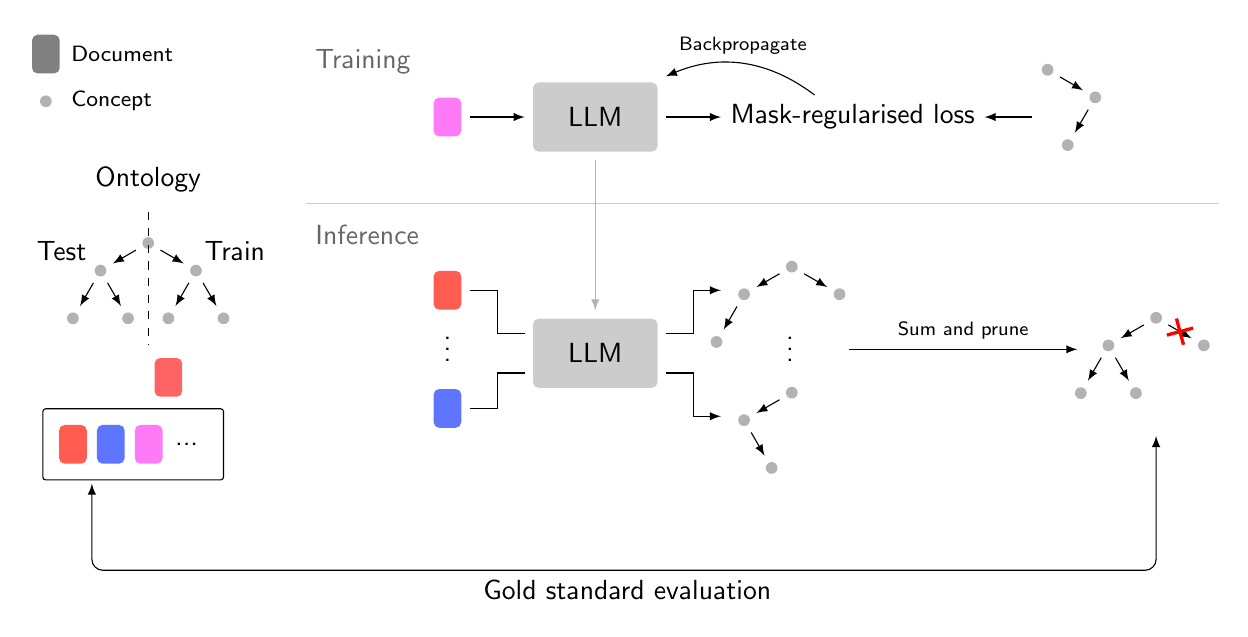
\begin{tikzpicture}
        [
            >=latex,
            doc/.style={
                    rectangle,
                    rounded corners=2pt,
                    % fill={black!80},
                    minimum width=10pt,
                    minimum height=14pt,
                    outer sep=3pt,
                },
            llm/.style={
                    rectangle,
                    rounded corners=2pt,
                    fill={black!20},
                    minimum width=45pt,
                    minimum height=25pt,
                    outer sep=3pt,
                },
            concept/.style={
                    circle,
                    fill={black!30},
                    inner sep=1.5pt,
                    outer sep=3pt,
                },
            every node/.append style={font=\sffamily},
            pics/.cd,
            % Marque croix en diagonale
            Cross/.style args={#1 and #2}{%
                    code = {%
                            \draw[#2,rotate=45,scale=1.4,very thick]
                            (0,#1 pt) -- (0,-#1 pt) ;
                            \draw[#2,rotate=-45,scale=1.4,very thick]
                            (0,#1 pt) -- (0,-#1 pt) ;
                        }
                },
            Cross/.default={2.5 and gray!25!black},
        ]
        \newcommand{\nodeDist}{0.7}
        \newcommand{\angleA}{30}
        \newcommand{\angleB}{60}
        \definecolor{c1}{RGB}{255,93,82}
        \definecolor{c2}{RGB}{94,118,255}
        \definecolor{c3}{RGB}{255,122,246}
        \definecolor{c4}{RGB}{255,100,100}

        % PART A: Ontology
        \node[concept] (root) {};
        \node[concept] (l1) at ($(root) + ({180+\angleA}:{\nodeDist})$) {};
        \node[concept] (l2) at ($(root) + ({-\angleA}:{\nodeDist})$) {};
        \node[concept] (l11) at ($(l1) + ({180+\angleB}:{\nodeDist})$) {};
        \node[concept] (l12) at ($(l1) + ({-\angleB}:{\nodeDist})$) {};
        \node[concept] (l21) at ($(l2) + ({180+\angleB}:{\nodeDist})$) {};
        \node[concept] (l22) at ($(l2) + ({-\angleB}:{\nodeDist})$) {};
        \draw[->] (root) -- (l1);
        \draw[->] (root) -- (l2);
        \draw[->] (l1) -- (l11);
        \draw[->] (l1) -- (l12);
        \draw[->] (l2) -- (l21);
        \draw[->] (l2) -- (l22);

        \newcommand{\docSpace}{0.2}
        \node[align=center] (caption) at ($(root) + (0, 0.8)$) {Ontology};
        \node[doc,fill=c1] (doc1) at ($(l11) + (0, -1.6)$) {};
        \node[doc,fill=c2] (doc2) at ($(doc1.east) + (\docSpace, 0)$) {};
        % \node[doc,fill=c3] (doc3) at ($(doc2.east) + (\docSpace, 0)$) {};
        \node[doc,fill=c3] (doc3) at ($(doc2.east) + (\docSpace, 0)$) {};
        \node[doc] (dots3) at ($(doc3.east) + (\docSpace, 0)$) {...};
        \draw[rounded corners=1pt] ($(doc1.north west) + (-0.1, 0.1)$) rectangle ($(dots3.south east) + (0.1, -0.1)$);

        % \newcommand{\docSpace}{0.75}
        % \node[doc,fill=c1] (doc1) at ($(l11) + (-0.2, -\docSpace)$) {};
        % \node[doc,fill=c2] (doc2) at ($(l12) + (0, -\docSpace)$) {};
        \node[doc,fill=c4] (doc4) at ($(l21) + (0, -0.75)$) {};
        % \draw[densely dashed] ($(l11)!0.5!(l12)$) -- ($(doc1)!0.5!(doc2)$);
        % \node at ($(doc1)!0.5!(doc2)$) {...};
        % \draw[densely dashed] (l11) -- (doc1);
        % \draw[densely dashed] (l12) -- (doc2);
        % \draw[densely dashed] (l21) -- (doc3);

        % line to separate the ontology into train and test
        \draw[dashed] ($(root) + (0, 0.4)$) -- ($(root) + (0, -1.3)$);
        \node at ($(root) + (1.1, -0.1)$) {Train};
        \node at ($(root) + (-1.1, -0.1)$) {Test};

        % PART B: Training
        \newcommand{\trainSpace}{0.7}
        \node[doc,fill=c3] (input) at ($(root) + (3.8, 1.6)$) {};
        \node[llm,anchor=west] (llm) at ($(input.east) + (\trainSpace, 0)$) {LLM};
        \node[anchor=west,align=center] (loss) at ($(llm.east) + (\trainSpace, 0)$) {Mask-regularised loss};
        \node[concept] (sgRoot) at ($(loss.east) + (\trainSpace + 0.1, 0.6)$) {};
        \node[concept] (sg2) at ($(sgRoot) + ({-\angleA}:{\nodeDist})$) {};
        \node[concept] (sg21) at ($(sg2) + ({180+\angleB}:{\nodeDist})$) {};
        \draw[->] (input) -- (llm);
        \draw[->] (llm) -- (loss);
        \draw[->] ($(loss.east) + (\trainSpace-0.1, 0)$) -- (loss);
        \draw[->] (sgRoot) -- (sg2);
        \draw[->] (sg2) -- (sg21);
        \draw[->,bend right] (loss) to node [midway,above,align=center] {\scriptsize Backpropagate} (llm);

        % PART C: Inference
        \node[llm] (llm1) at ($(llm) + (0, -3.0)$) {LLM};
        \node[doc,fill=c1,anchor=east] (input1) at ($(llm1.west) + (-\trainSpace, 0.8)$) {};
        \node[concept] (sgRoot1) at ($(llm1.east) + (\trainSpace + 0.9, 1.1)$) {};
        \node[concept] (sg11) at ($(sgRoot1) + ({180+\angleA}:{\nodeDist})$) {};
        \node[concept] (sg12) at ($(sgRoot1) + ({-\angleA}:{\nodeDist})$) {};
        \node[concept] (sg111) at ($(sg11) + ({180+\angleB}:{\nodeDist})$) {};
        \node[doc,fill=c2,anchor=east] (input2) at ($(llm1.west) + (-\trainSpace, -0.7)$) {};
        \node[concept] (sgRoot2) at ($(llm1.east) + (\trainSpace + 0.9, -0.5)$) {};
        \node[concept] (sg21) at ($(sgRoot2) + ({180+\angleA}:{\nodeDist})$) {};
        \node[concept] (sg212) at ($(sg21) + ({-\angleB}:{\nodeDist})$) {};
        \node (dots) at ($(input1)!0.5!(input2) + (0, 0.1)$) {$\vdots$};
        \node (dots2) at ($(dots) + (4.35, 0)$) {$\vdots$};
        \newcommand{\vertSpace}{0.25}
        \draw (input1) -| ($(input1.east)!0.5!(llm1.west)$) |- ($(llm1.west) + (0, \vertSpace)$);
        \coordinate (out1) at ($(llm1.east) + (\trainSpace, 0.8)$);
        \draw[->] ($(llm1.east) + (0, \vertSpace)$) -| ($(llm1.east)!0.5!(out1)$) |- (out1);
        \draw (input2) -| ($(input2.east)!0.5!(llm1.west)$) |- ($(llm1.west) + (0, -\vertSpace)$);
        \coordinate (out2) at ($(llm1.east) + (\trainSpace, -0.8)$);
        \draw[->] ($(llm1.east) + (0, -\vertSpace)$) -| ($(llm1.east)!0.5!(out2)$) |- (out2);


        % \node[doc,fill=c1] (input1) at ($(input) + (0, -2.0)$) {};
        % \node[llm] (llm1) at ($(input1) + (\trainSpace, 0)$) {LLM};
        % \node[concept] (sgRoot1) at ($(llm1) + (\trainSpace + 0.8, 0.6)$) {};
        % \node[concept] (sg11) at ($(sgRoot1) + ({180+\angleA}:{\nodeDist})$) {};
        % \node[concept] (sg12) at ($(sgRoot1) + ({-\angleA}:{\nodeDist})$) {};
        % \node[concept] (sg111) at ($(sg11) + ({180+\angleB}:{\nodeDist})$) {};
        % \draw[->] (input1) -- (llm1);
        % \draw[->] (llm1) -- ($(llm1) + (\trainSpace-0.25, 0)$);
        \draw[->] (sgRoot1) -- (sg12);
        \draw[->] (sgRoot1) -- (sg11);
        \draw[->] (sg11) -- (sg111);

        % \node[doc,fill=c2] (input2) at ($(input1) + (0, -1.7)$) {};
        % \node[llm] (llm2) at ($(input2) + (\trainSpace, 0)$) {LLM};
        % \node[concept] (sgRoot2) at ($(llm2) + (\trainSpace + 0.8, 0.6)$) {};
        % \node[concept] (sg21) at ($(sgRoot2) + ({180+\angleA}:{\nodeDist})$) {};
        % \node[concept] (sg212) at ($(sg21) + ({-\angleB}:{\nodeDist})$) {};
        % \draw[->] (input2) -- (llm2);
        % \draw[->] (llm2) -- ($(llm2) + (\trainSpace-0.25, 0)$);
        \draw[->] (sgRoot2) -- (sg21);
        \draw[->] (sg21) -- (sg212);

        \node[concept] (testOutRoot) at ($(input1)!0.5!(input2) + (9.0, 0.4)$) {};
        \node[concept] (testOut1) at ($(testOutRoot) + ({180+\angleA}:{\nodeDist})$) {};
        \node[concept] (testOut11) at ($(testOut1) + ({-\angleB}:{\nodeDist})$) {};
        \node[concept] (testOut12) at ($(testOut1) + ({180+\angleB}:{\nodeDist})$) {};
        \node[concept] (testOut2) at ($(testOutRoot) + ({-\angleA}:{\nodeDist})$) {};
        \draw[->] (testOutRoot) -- (testOut1);
        \draw[->] (testOut1) -- (testOut11);
        \draw[->] (testOut1) -- (testOut12);
        \draw[->] (testOutRoot) -- pic[midway,-,rotate=-\angleA] {Cross={3.5 and red}} (testOut2);
        \draw[->] ($(input1)!0.5!(input2) + (5.1, 0)$) -- node [midway,above,align=center] {\scriptsize Sum and prune} ($(input1)!0.5!(input2) + (8.0, 0)$);

        % PART D: Evaluation
        \coordinate (start) at ($(doc1)!0.5!(doc2) + (0, -0.5)$);
        \coordinate (inter) at ($(start) + (6.8, -1.1)$);
        \coordinate (end) at ($(testOutRoot) + (0, -1.5)$);
        \draw[<->,rounded corners] (start) |- (inter) -| (end);
        \node[below] at (inter) {Gold standard evaluation};

        % Draw a separation line between Part B and Part C
        \draw[color={black!20}] ($(input)!0.5!(input1) + (-1.8, 0)$) -- ($(input)!0.5!(input1) + (9.8, 0)$);
        % Caption Part B
        \node[color={black!60},anchor=west] at ($(input)!0.5!(input1) + (-1.8, 1.8)$) {Training};
        % Caption Part C
        \node[color={black!60},anchor=west] at ($(input)!0.5!(input1) + (-1.8, -0.4)$) {Inference};
        % Arrow connection llm train to llm inference.
        \draw[->,color={black!30}] (llm) -- (llm1);
        % Legend
        \node[doc,fill={black!50}] (docLegend) at ($(root) + (-1.3, 2.4)$) {};
        \node[anchor=west] (docDesc) at ($(docLegend) + (0.2, 0)$) {\footnotesize Document};
        \node[concept] (conceptLegend) at ($(docLegend) + (0, -0.6)$) {};
        \node[anchor=west] (conceptDesc) at ($(conceptLegend) + (0.2, 0)$) {\footnotesize Concept};
    \end{tikzpicture}

    \caption{Overview of \name. A finetuned LLM is used to model the relevant subgraph for each document in the source corpus. The generated subgraphs (sub-ontologies) are then summed into a weighted graph, and pruning is applied to obtain the final output ontology.}
    \label{fig:overview}
\end{figure}

I introduce \name, an end-to-end method for using LLMs to construct ontologies at scale. Rather than focusing on individual relations between concepts, I finetune an LLM to model entire sub-components of the target ontology. The output ontology is generated by taking the sum of generated sub-components and applying simple post-processing. An overview of the pipeline is shown in \cref{fig:overview}. To train \name, I collect the categorisation metadata for a subset of Wikipedia articles. I attempt to adapt an LLM to model the relevant categorisation subgraph for a particular Wikipedia article, but discover that direct finetuning leads to poor generalisation due to overfitting to high-level, frequently occurring concepts. Instead, I propose a custom regulariser that reweights each concept based on its frequency of occurrence, which substantially improves generalisation.

I evaluate \name by measuring the similarity of the generated ontology with the ground truth. Current approaches for comparing ontologies rely on mapping classes of the two ontologies onto each other, most commonly by literal text matching. \todo{Add citation} This is unreliable when the two ontologies are not already sufficiently similar. Instead, I propose a suite of evaluation metrics suitable for comparing arbitrary labelled graphs. These metrics compare edges and subgraphs of the two ontologies using pretrained text embedders to test for semantic and structural similarity. The results reveal that an LLM can already outperform existing extraction-based methods out of the box, and the performance can be further improved by finetuning with our custom regulariser. I additionally demonstrate that \name can be adapted to build the arXiv ontology using only a small number of training examples, suggesting that our model can be applied to new domains in a data-efficient way.

\textbf{Contributions}
\begin{enumerate}
    \item I constructed two datasets based on Wikipedia and arXiv, which can serve as standard datasets for future work studying end-to-end OL.
    \item I created \name, a method that utilises LLMs to build ontologies from scratch. \name produces high-quality ontologies and serves as a strong baseline for end-to-end OL.
    \item I developed new evaluation metrics for end-to-end OL.
\end{enumerate}


\chapter{Background}

This project's research topic is in the intersection of ontology learning, ontology evaluation, and large language models for structured knowledge representation. This chapter provides an overview of the standard techniques and core principles in these areas, and discusses potential research gaps that this project aims to address.

\section{What is an ontology?}

% [What is an ontology and how is it represented?]
An ontology is a structured way of representing concepts and relations of a shared conceptualisation, i.e. domain knowledge \cite{gruber1995toward,gruber1993translation}. The primary goal of an ontology is to represent the entities in a domain in a machine-readable format and linking the relationships among them \cite{national2022ontologies}. This project focuses on ontologies that only consist of concepts and taxonomic relations which represent \emph{is-a} or \emph{is-subclass-of} relationships between concepts. In some cases, the \emph{is-part-of} relation is also considered a taxonomic relation.

% [Representations of ontologies]
We treat such an ontology as a rooted labelled directed graph where nodes represent concepts, edges represent taxonomic relations and the root node is the special concept of all concepts. A strict ontology asserts that the taxonomic relation is asymmetric and thus the graph must be acyclic, though in practice some ontologies, such as the Wikipedia ontology studied in this paper, may contain cycles. We therefore do not assume that an ontology graph is necessarily acyclic. Examples of ontologies include WordNet \cite{miller1995wordnet} with 117,659 concepts and 89,089 taxonomic relations and the Gene Ontology \cite{ashburner2000gene} with 42,255 concepts and 66,810 taxonomic relations.

\section{Ontology learning}

% [What is the precise task we study in this paper?]
Ontology learning is the automatic extraction of ontological elements \cite{hazman2011survey}. The most studied source of input is unstructured text, though there are also works on OL on semi-structured data like HTML \cite{karoui2004ontology}. In this paper, the input is a set of documents, each consisting of some unstructured text. We additionally assume each document is associated with one or more concepts in the ground truth ontology which we utilise for training. The goal is to reconstruct the ground truth ontology given the set of documents.

\subsection{Hearst patterns}  \label{sec:hearst}

% [Traditional approaches to OL.]
Prior works view OL as a composition of subtasks and study each subtask in isolation \cite{buitelaar2005ontology,asim2018survey}. A typical pipeline for building a simple ontology is to first perform concept discovery (identify the nodes) and then relation extraction (identify the edges) \cite{cimiano2005text2onto,kaushik2018automatic}. A notable approach for relation extraction is Hearst patterns \cite{hearst1998automated}. Hearst patterns are hand-crafted lexico-syntactic patterns that exploit natural language structure to discover taxonomic relations. For example, the pattern ``NP such as NP'' matches phrases like ``dogs such as chihuahuas'' and thus can be processed by regular expressions to identify the relation ``dog $\to$ chihuahua''. Hearst patterns suffer from low recall as the relations must occur in exact configurations to be matched by rules. More recent works have suggested smoothing techniques to alleviate this issue \cite{roller2018hearst}.
% Another approach for relation extraction utilises word co-occurrence statistics to predict taxonomic relations \cite{cimiano2005learning}.

% [LLM approaches to OL]
Recent research has transitioned to using language models for OL. REBEL \cite{cabot2021rebel} treats relation discovery as a translation task and finetunes encoder-decoder LLMs to extract both taxonomic and non-taxonomic relations. \citet{babaei2023llms4ol} benchmarked a wide family of LLMs for concept and relation discovery and showed promising results. There are also proof-of-concept works for building ontologies end-to-end with LLMs. \citet{funk2023towards} proposes to build an ontology by recursive prompting an LLMs while \citet{trajanoska2023enhancing} generates the entire ontology in one completion. However, both studies are limited in the scale of the task and evaluation. The authors only considered ontologies of up to 1000 concepts and relied on manual qualitative evaluation. We bridge this gap by proposing a method that can scale to practical problem sizes and new metrics for systematic qualitative evaluation.

\section{Evaluating ontologies}

% [Prior approaches to evaluating OL.]
The evaluation of ontologies is also an open research area. The main approaches are gold-standard evaluation, which matches elements of the generated ontology with a predefined target ontology; task-based evaluation, which measures the usefulness of the ontology on a specific application; and human evaluation \cite{raad2015survey,brank2005survey}. In this paper, we evaluate by the gold standard as it is the most straightforward approach when such ground-truth ontology exists. Prior works have considered matching concepts \cite{maedche2002measuring} and direct and indirect relations \cite{Kashyap2005TaxaMinerAE, Treeratpituk2013GraphbasedAT} by literal text comparison. Other works have also considered edit-distance \cite{Ehrig2005SimilarityFO} or bag-of-words distributional similarity for text comparison \cite{Zavitsanos2011GoldSE}.  These techniques may be considered unreliable and have been superseded by current methods \cite{conneau2017supervised}. We instead rely on more modern techniques like pretrained text embedders \cite{devlin2018bert} and graph convolutions \cite{kipf2016semi} to match substructures between the two ontologies.

\section{LLMs for knowledge representation}

Outside of OL, there is a growing body of research on using LLMs to construct structured knowledge representations, most commonly as \emph{knowledge graphs} (KGs) \cite{singhal2012introducing}. While ontologies focuses on capturing the relationship between concepts, KGs aims to represent \emph{instances} of such concepts and their properties \cite{guarino1995ontologies}. For example, an ontology may capture the common sense relation that ``a person is born at a place'', while a knowledge graph might contain explicit instantiations like ``Barack Obama is born in Honolulu''. As a result, the construction of KGs focuses more on extracting facts from the source corpus and less on the structure of the graph itself.

Similar to OL, knowledge graph construction is rarely studied in an end-to-end framework. Instead, most works focus on subtasks such as entity prediction: discover which entities should be in the KG; link prediction: classify whether two entities are related by a specified relation; and KG completion: given a head node and a relation, predict the tail node. \todo{Add citations} The first work to use LLMs for KG completion is \citet{petroni2019language}, who demonstrated that many facts can be elicited by simply prompting a LLM with a relation and a head entity. Recent works have further explored the use of LLMs for KG construction, such as \citet{yao2023exploring} who finetuned LLMs for link prediction and relation prediction, and \citet{wang2020language} who inspected the attention patterns of LLMs to extract the relation token(s) between two entities in the source text. While these works have shown promising results, they do not address the research questions of this project, in particular whether are any benefits to studying knowledge representations tasks in an end-to-end manner. While the primary focus of this project is OL, the results have extended implications for KG construction as well.

\section{Graph analysis}

Since we treat ontologies as graphs in this project, standard graph analysis techniques are applicable too. In particular, these ideas will become relevant when we design metrics for analysing and evaluating the generated ontologies. This section explains two key concepts used in this project: \emph{network motifs} and \emph{node embeddings}.

\subsection{Network motifs}

Network motifs are recurring subgraphs that appear more frequently in a graph than in a random graph \cite{milo2002network}. Studying the frequency or the location of the motifs in a graph can provide insights into the graph's global structures. For example, the fully-connected three-vertex graph is a motif commonly found in social networks \cite{stone2019network}, indicating the general property that if Alice is friends with Bob and Bob is friends with Charlie, then Alice and Charlie are likely to be friends as well. More generally, motif analysis is an instantiation of \emph{graphlet counting} \cite{ribeiro2021survey} which aims to compute the frequency of all possible subgraphs of a certain size. Graphlet counting has been used to evaluate graph generation models \cite{you2018graphrnn} by comparing the $n$-node graphlet counts between two graph distributions. In this project, however, we are interested in comparing two specific graph instances (the generated ontology versus the ground truth) hence such metrics do not directly apply.

\subsection{Node embeddings}

Node embeddings are vector representations of the nodes in a graph that aims to summarise their graph position and the structure of their local graph neighbourhood \cite{hamilton2020graph}. Node embeddings are useful for many graph analysis tasks, such as node classification and link prediction. One of the most popular algorithms for generating node embeddings is node2vec \cite{grover2016node2vec}, which uses random walks to sample the relevant neighbourhood around each node and optimises the embeddings to be predictive of whether two nodes are neighbours. It is however only designed for graphs where nodes are unlabelled (also known as \emph{homogenous graphs}) and thus not suitable for ontologies.

A method suitable for learning node embeddings for labelled graphs are \emph{graph convolutions}. Suppose for a graph $G = (V, E)$, we have $\m{A}$ its adjacency matrix and the node feature (label) matrix $\m{X} \in \R^{|V| \times d}$, where $d$ is the feature dimension. The graph convolution operator with parameters $\m{W} \in \R^{d \times d}$ is defined as
\[
    \m{X}' = \hat{\m{D}}^{-1/2} \hat{\m{A}} \hat{\m{D}}^{-1/2} \m{X} \m{W}
\]
where $\hat{\m{A}} = \m{A} + \m{I}$ and $\hat{D}_{ii} = \sum_j \hat{A}_{ij}$ the diagonal degree matrix. Intuitively, applying a graph convolution to $\m{X}$ aggregates the features of each node's 1-hop neighbourhood and applies a linear transformation to the result. A simple yet effective extension to gather information from further neighbours without introducing more parameters is known as a \emph{simple graph convolution} \cite{wu2019simplifying}:
\begin{equation}  \label{eq:simple-graph-conv}
    \m{X}' = \left(\hat{\m{D}}^{-1/2} \hat{\m{A}} \hat{\m{D}}^{-1/2}\right)^K \m{X} \m{W}
\end{equation}
where $K$ determines the number of hops. A weakness of simple graph convolutions is that they are prone to \emph{over-smoothing} \cite{zhu2020simple}, where node embeddings become increasing generic and thus uninformative as $K \to \infty$. Empirically, using small values of $K$ (e.g. $K = 2$) tends to be the most effective \cite{wu2019simplifying}.

\chapter{Design and implementation}

One of the goals of this project is to explore the paradigm shift from traditional subtask composition OL to end-to-end OL. The novelty of the task in of itself means that many components of the project has to be built from ground up. This chapter documents the implementation and design decisions made for each of these building blocks, including curating the datasets (\cref{sec:implementation:data-collection}), building reliable baselines (\cref{sec:implementation:baselines}), introducing our own method \name (\cref{sec:implementation:core}), and developing robust methods of evaluation (\cref{sec:implementation:evaluation}).

% \section{Starting point}

% This project is not based on any existing codebase. The Wikipedia and arXiv datasets to be used in this project are also not readily available. In addition, few prior works in OL have open-source implementation, even including unofficial ones. Knowing the novelty of the end-to-end OL task studied in this project, I decided to build the project from scratch as it would give me to the most flexibility in designing the system.

\section{Data collection}  \label{sec:implementation:data-collection}

Two datasets are used in this project: Wikipedia categories and the arXiv taxonomy. Wikipedia is chosen as its categorisation metadata is entirely human-annotated by Wikipedia maintainers and authors while simultaneously being large and diverse. This makes it a good candidate base dataset for training and evaluation. The arXiv taxonomy on the other hand is much smaller and simpler than Wikipedia. Ontologies of this size is much easier to manually inspect and understand, making it a good candidate for evaluation. In addition, the papers on arXiv are written in a different style than Wikipedia articles, and so we can evaluate the out-of-domain generalisation ability of our model by testing it on arXiv. While both data sources are in the public domain, there are no readily available datasets that contain both the main text and the categorisation metadata. I therefore have to build the datasets from scratch.

\subsection{Wikipedia}

\subsection{arXiv}

We collect the datasets for the two ontologies considered in this paper: Wikipedia categories and the arXiv taxonomy. We use Wikipedia for learning and in-domain evaluation and arXiv for out-of-domain evaluation. To build the Wikipedia dataset, we perform a BFS traversal from its root category ``Main topic classifications'' up to depth 3. For every category encountered, we retrieve the title and summary (the text before the first section) of up to 5000 pages that belong in that category. The source data is obtained from the Wikipedia API.\footnote{\url{https://en.wikipedia.org/w/api.php}} The arXiv taxonomy is available from its home page and the source corpus is constructed from the title and abstract of all the papers uploaded to arXiv in the years 2020--2022 with more than or equal to 10 citations.\footnote{Citation counts obtained from \url{https://api.semanticscholar.org/}.} In total, the Wikipedia dataset has 13,886 concepts, 28,375 taxonomic relations and 362,067 documents, while the arXiv dataset has 161 concepts, 166 taxonomic relations and 126,001 documents.

\section{Baselines}  \label{sec:implementation:baselines}

We give a brief overview of the baseline methods here. The full implementation details can be found in \cref{appendix:exp-details}. All baselines produce weighted directed graphs which we apply the same post-processing steps as \name (\cref{sec:method:post-processing}) to obtain the final predicted graph.

\paragraph{Memorisation}
Simply memorising the train graph is a surprisingly strong baseline due to the overlap between train and test graphs, especially for Wikipedia. The weight of each edge is given by the number of relevant subgraphs in which it appears.

\paragraph{Hearst}
We follow the improved implementation of Hearst patterns by \citet{roller2018hearst}. The authors propose spmi, a method which uses low-rank approximations to smooth the relation matrix so that two concepts can be compared even if there are no direct matches between them. We use the smoothed relation matrix to weigh the relations between the ground truth concepts. The additional hyperparameter for the rank of the smoothed matrix is tuned by grid search over the validation set.

\paragraph{REBEL}
The REBEL-large model \cite{cabot2021rebel} is an encoder-decoder LLM trained to extract many types of relations from Wikipedia articles. We only take the ``subclass of'', ``instance of'', ``member of'' and ``part of'' relations that were extracted. Similar to \textbf{Hearst}, we find that it fails to find many direct relations between ground truth concepts. The same low-rank smoothing technique is applied to give a higher recall.

\paragraph{Prompting}
We test the \textbf{zero/one/three-shot} performance of instruction-tuned LLMs on the subgraph modelling task described in \cref{sec:method:subgraph}. We use Mistral 7B Instruct v0.2 \cite{jiang2023mistral} as the instruct model. We perform manual prompt engineering to describe the task and steer the model to return outputs of the same format as that described in \cref{sec:method:subgraph}. The prompt can be found in \cref{appendix:prompt-template}.


\section{\name}  \label{sec:implementation:core}

This section introduces \name, a simple and scalable method for end-to-end OL with LLMs. On a high level, \name uses an LLM to model linearised subgraphs of the target ontology. In contrast to learning individual edges, modelling subgraphs allows the model to learn higher-order structures, such as the interactions between three or more nodes. To create the training dataset, \name relies on the assignment of documents to concepts which induces a relevant subgraph for each document. Such subgraphs are much smaller than the complete graph so they can be learned by the model more easily. The generated subgraphs for each document are summed into a weighted graph and simple post-processing is applied to obtain the final predicted ontology.

% Highlight the core components and insights for \name.
% \begin{enumerate}
%     \item The idea to model subgraphs instead of edges. Motivation: More efficient inference, captures the global structure of an ontology (the hierarchical structure is "baked in").
%     \item Components: 1. Document $\to$ subgraph. 2. Aggregrate subgraphs induced by each document into a weighted global graph. 3. Apply post-processing and pruning.
%     \item Argue that this setup is appealing for scaling: Inference can be parallelised across the source documents, so inference duration is inversely proportional to the amount of hardware available. 
% \end{enumerate}

\subsection{Subgraph modeling}  \label{sec:method:subgraph}

\begin{figure}[t]
    \centering
    \begin{subfigure}[c]{0.34\textwidth}
        \centering
        \fbox{
        \includegraphics[width=\linewidth,trim={1.5cm 1.5cm 1.5cm 1.5cm},clip]{media/Hybridity.pdf}
        }
    \end{subfigure}%
    \hfill
    \begin{adjustbox}{varwidth=\linewidth,fbox}
    \begin{subfigure}[c]{0.55\textwidth}
        \centering
        \lstdefinestyle{prompt}{
          basicstyle=\small\ttfamily\color{black},
          moredelim=**[is][\color{gray}]{@}{@},
        }
        \begin{lstlisting}[gobble=8,style=prompt]
        @<s>[INST] Title: Hybridity
        Hybridity, in its most basic sense ... [/INST]@
        Main topic classifications -> @Human behavior@ -> @Human activities@ -> Culture -> Sociology of culture
        Main topic classifications -> @Humanities@ -> Politics -> @Politics by issue@ -> @Politics and race@
        Main topic classifications -> @Politics@ -> @Politics by issue@ -> Politics and race
        Main topic classifications -> @Culture@ -> Sociology of culture</s>
        \end{lstlisting}
    \end{subfigure}
    \end{adjustbox}
    \caption{Example subgraph induced by the Wikipedia page ``Hybridity'' (left), where $N = 4$ and $C = \{\text{Politics and race}, \text{Sociology of culture}\}$.
    The corresponding training text sequence (right), where text coloured in grey is ignored as training targets but is still present as context for later tokens.}
    \label{fig:prompt-template}
\end{figure}

Here, we describe the method for creating document-subgraph pairings. Given a document and its associated set of concepts $C$, we define the \emph{relevant paths} as the set paths of at most length $N$ from the root to any of the concepts in $C$. The \emph{relevant subgraph} is the set of nodes and edges that occur at least once in the relevant paths. An example is shown in the left subfigure of \cref{fig:prompt-template}. The choice of $N$ is task-specific and we describe our method for choosing $N$ in \cref{sec:implementation}.

To employ LLMs to model the subgraphs, we must linearise the graph into a string for sequence modelling. Existing methods for autoregressive graph generation employ BFS \cite{you2018graphrnn} or DFS \cite{goyal2020graphgen} ordering starting at an arbitrary node. We instead choose to linearise the subgraph as a list of relevant paths that produced the subgraph in the first place. We do so for three reasons: Firstly, the subgraph is defined from such a collection of paths which makes them the most natural representation; Secondly, we hypothesise the hierarchy of concepts on each path is a desirable inductive bias for the hierarchical nature of an ontology; Thirdly, the path-based representation is much easier to describe in natural language instructions so that our LLM prompting-based baselines may produce reasonable results without finetuning. The linearisation template can be found in \cref{appendix:prompt-template}.

% Key points:
% \begin{enumerate}
%     \item Explain how to construct document-subgraph pairing from the training dataset. E.g., the path length cutoff is selected as the smallest number that still covers almost all of the edges.
%     \item Linearisation of subgraph to a sequence. Why choose the method of ``subgraph as a set of paths''? Ans: More natural language-like, easier for zero/few-shot to comprehend so we have stronger baselines.
%     \item \fig{Example output format.}
% \end{enumerate}

\subsection{Post-processing}  \label{sec:method:post-processing}

The final output graph is obtained by summing all generated subgraphs for each document and pruning low-weighted components. Given the generated subgraphs $G_1 = (V_1, E_1), \dots, G_n = (V_n, E_n)$, the raw output graph is defined as $G_{\text{raw}} = (V_{\text{raw}}, E_{\text{raw}})$ where $V_\text{raw} = \cup_{i=1}^n V_n$ and $E_\text{raw} = \cup_{i=1}^n E_n$. Each edge $(u, v) \in E_\text{raw}$ is additionally weighted by the number of times they occur in the collection of subgraphs: $w_{u, v} = \sum_{i=1}^n \mathbb{1}[(u,v) \in E_n]$. A few simple post-processing steps are then applied to $G_\text{raw}$:
\begin{enumerate}
    \item Self-loop pruning: All edge $(u, u) \in E_\text{raw}$ are removed.
    \item Inverse-edge pruning: All edges $(u, v) \in E_\text{raw}$ where $(v, u) \in E_\text{raw}$ and $w_{v, u} > w_{u, v}$ are removed.
    \item Absolute thresholding: Edges in $E_\text{raw}$ with weight below the $\alpha$-th quantile are removed, where $0 \leq \alpha \leq 1$ is a hyperparamter.
    \item Relative thresholding: For each vertex $u \in V_\text{raw}$, let $e_1, \dots, e_k$ be the outgoing edges from $u$ sorted by weight in ascending order. Define the cumulative weight as $C(e_i) = \sum_{j=1}^i w_{e_j} / \sum_{j=1}^k w_{e_j}$. The edges $\{e_i\ |\ C(e_i) \leq \beta\}$ are pruned, where $0 \leq \beta \leq 1$ is a hyperparameter.
    \item Clean up: After pruning all edges, nodes with no incoming or outgoing edges are removed.
\end{enumerate}
In our implementation, we choose the hyperparameters $\alpha$ and $\beta$ by tuning on the validation set.

% Key points:
% \begin{enumerate}
%     \item Aggregate inference outputs into a weighted directed graph.
%     \item Following \cite{roller2018hearst}, we prune self loops and edge $u \to v$ if $v \to u$ is also in the graph with a higher weight.
%     \item Apply two thresholding values to prune the graph further. The first threshold $\alpha$ where the lowest-weighted $100 \alpha\%$ of edges are pruned. The second threshold $\beta$ is a relative threshold where \emph{for each node}, the lowest-weighted outgoing edges that are in the bottom $100\beta\%$ cumulative probability mass are removed. \todo{Perhaps easier to describe in equations.}
%     \item The hyperparameters $\alpha$ and $\beta$ are tuned on the evaluation set.
% \end{enumerate}

\section{How to evaluate end-to-end OL?}  \label{sec:implementation:evaluation}

Since our problem setup is uncommon in existing literature, we also develop new evaluation methods. Ontology evaluation is a hard problem as there are no quantitative definitions of what constitutes a ``good ontology'' and metrics generally only capture one aspect of an ontology. We approach evaluation by treating the ground truth as a proxy for a good ontology and comparing the generated ontologies against the ground truth. This section describes how the ground truth is obtained and what metrics are used for measuring ontology similarity.

% Key points:
% \begin{enumerate}
%     \item Explain the goals of evaluation---what do we care about? Ans: Semantics and structure.
%     \item Suggest why end-to-end evaluation is hard: Large graph. Generally, a ``good ontology'' is ill-defined. Difficult to find one metric that describes all. Always trade-offs. No standard evaluation metric. 
%     \item How do we overcome this? 1. Use a ground truth ontology as a proxy for ``good ontology'' and measure how similar the generated ontology is to the ground truth. 2. Propose a series of evaluation metrics to capture various aspects of the generated output.
% \end{enumerate}

\subsection{Create train and test splits}

\begin{figure}
    \centering
    \begin{subfigure}[t]{0.3\linewidth}
        \centering
        \includegraphics[width=\linewidth,trim={0.4cm 0.65cm 0.5cm 0.9cm},clip]{media/Wikipedia_train_eval_test_split.pdf}
        \caption{Wikipedia}
    \end{subfigure}%
    \qquad\qquad
    \begin{subfigure}[t]{0.25\linewidth}
        \centering
        \includegraphics[width=\linewidth,trim={1cm 1cm 1cm 1.2cm},clip]{media/arXiv_train_eval_test_split.pdf}
        \caption{arXiv}
    \end{subfigure}
    \caption{Intersection of concepts among the train, validation and test splits of the datasets.}
    \label{fig:dataset-overlap}
\end{figure}


Generating the train and test splits from the datasets is also a non-trivial problem. As described in \cref{sec:method:subgraph}, each training example consists of a document and its induced subgraph. The naive approach of randomly selecting a subset of documents for the training set likely leads to data leakage as there might be a significant overlap between subgraphs in the training set and the test set. Instead, we propose to first split the full ontology in train and test graphs and then generate the training document-subgraph pairs. Our method is as follows:
\begin{enumerate}
    \item Let $V^\text{top}$ be the set of top-level nodes, i.e. children of the root node. Randomly partition $V^\text{top}$ into train $V^\text{top}_{\text{train}}$, validation $V^\text{top}_{\text{val}}$, and test $V^\text{top}_{\text{test}}$ splits in 7:3:10 ratio.
    \item Let $d$ be the depth on the full graph, i.e. the distance of the furthest node from the root. The nodes of the train graph are taken as the union of all the nodes that are within distance $d - 1$ from any node in $V^\text{top}_\text{train}$, plus $V_\text{train}^\text{top}$ and the root. The edges are all the edges in the full graph that have both endpoints in the train graph. Similar applies for $V^\text{top}_\text{val}$ and $V^\text{top}_\text{test}$.
\end{enumerate}
Our methods ensure that there are sufficiently many unseen concepts (and thus relations) in the test split, as shown in \cref{fig:dataset-overlap}.

% Key points:
% \begin{enumerate}
%     \item Describe the data collection procedure.
%     \item Report the dataset statistics, e.g., number of nodes/edges/documents. Wikipedia: 13886 / 28375 / 362067. arXiv: 161 / 166 / 126001.
%     \item Highlight the thought process behind the creation of the train-eval-test split (Balance between the diversity of the training set and having unseen nodes/edges in the eval/test split).
%     \item \fig{Venn diagram to show the overlap between the train/eval/test splits. \cref{fig:dataset-overlap}}
% \end{enumerate}

\subsection{Metrics}

Existing methods for measuring similarity between ontologies rely on outdated techniques such as edit distance or document co-occurrence statistics for text comparison. To obtain more reliable evaluation results, we propose a suite of similarity metrics that uses more modern methods like text embeddings. Multiple metrics are used as they trade off interpretability with comprehensiveness, and we aim to make them complementary by capturing different aspects of an ontology. In this section, we denote the ground truth ontology graph as $G = (V, E)$ and the generated graph as $G' = (V', E')$.

\paragraph{Literal F1 \cite{Kashyap2005TaxaMinerAE}}
While literal text matching is unreliable, it is also the simplest and the most interpretable. The Literal F1 metric is given by the harmonic mean of the precision and recall of the edges:
\[
    \text{Literal precision} = \frac{|E \cap E'|}{|E'|} \qquad
    \text{Literal recall} = \frac{|E \cap E'|}{|E|}
\]

\paragraph{Fuzzy F1}
The literal F1 metric puts a strong emphasis on using the correct wording, while in practice, we are interested in evaluating the semantics of an ontology. For example, using a synonymous phrase for a concept should not be penalised. We utilise embeddings from a pretrained sentence transformer and use the cosine similarity of the embeddings to measure semantic similarity. Specifically, let $\nodesim(u, u') \in V \times V' \to [-1, 1]$ be the cosine similarity between the sentence embeddings for $u$ and $u'$. The Fuzzy F1 score is obtained from the fuzzy precision and recall, defined as:
\begin{equation*}
    \begin{aligned}
        \text{Fuzzy precision} & = \frac{|
            \{(u', v') \in E' \mid \exists (u, v) \in E.
            \nodesim(u, u') > t \land \nodesim(v, v') > t
            \}
        |}{|E'|}                           \\
        \text{Fuzzy recall}    & = \frac{|
            \{(u, v) \in E \mid \exists (u', v') \in E'.
            \nodesim(u, u') > t \land \nodesim(v, v') > t
            \}
        |}{|E|}                            \\
    \end{aligned}
\end{equation*}
where $t$ is the matching threshold. We use all-MiniLM-L6-v2 \cite{wang2020minilm,reimers-2019-sentence-bert} as the embedding model and choose $t$ as the median cosine similarity between the synonyms in WordNet \cite{miller1995wordnet}, computed to be 0.436.

\paragraph{Continuous F1}
With fuzzy comparisons, the matches between the edges of the generated and the ground truth graph are no longer one-to-one. This is problematic: Consider two graphs $A \rightarrow B$ and $B \leftarrow A \rightarrow B'$, where $B$ and $B'$ match fuzzily. Such graphs will achieve a perfect fuzzy F1 score yet they significantly differ. Additionally, we found that the previous metrics fail to provide a useful signal for hyperparameter tuning, particularly for our baselines where the generated graphs are poor. The continuous F1 metric solves these issues by computing the highest-scoring edge matching between the two graphs, where the similarity score between $(u, v)$ and $(u', v')$ is given by $\min(\nodesim(u, u'), \nodesim(v, v'))$. Obtaining such matching is equivalent to solving the linear assignment problem \cite{martello1987linear}, which can be computed by the Hungarian algorithm \cite{kuhn1955hungarian}. The Continuous F1 is obtained from the continuous precision and recall, given by:
\[
    \text{Continuous precision} = \frac{s_\text{cont}}{|E'|} \qquad
    \text{Continuous recall} = \frac{s_\text{cont}}{|E|}
\]
where $s_\text{cont}$ is the score achieved by the best edge matching.

\paragraph{Graph F1}
Instead of individual edges, this metric aims to capture the wider structure of the two graphs. Intuitively, we want to know how concepts are related to their local neighbourhood. We do so by using simple graph convolutions \cite{wu2019simplifying} with $K=2$ to compute graph-aware node embeddings after embedding each node with the pretrained embedder. Such embeddings in $G$ are compared against those in $G'$ by cosine similarity, and the highest-scoring node matching, similar to the continuous F1 metric, gives the graph similarity score. The Graph F1 is computed from the graph precision and recall, defined to be:
\[
    \text{Graph precision} = \frac{s_\text{graph}}{|V'|} \qquad
    \text{Graph recall} = \frac{s_\text{graph}}{|V|}
\]
where $s_\text{graph}$ is the score achieved by the best node matching.

\paragraph{Motif distance}
Taking inspiration from classical network analysis, we use \emph{network motifs} \cite{milo2002network,shen2002network} to evaluate the structural integrity of the generated graphs. Network motifs are reoccurring subgraphs in a larger graph, most commonly 3-vertex subgraphs. They are typically indicative of the structural characteristics of the full graph. We define the motif distance as the 1-Wasserstein distance between the distribution of all 3-vertex subgraphs in $G$ and $G'$.


\chapter{Evaluation}  \label{chap:evaluation}

In this chapter, we aim to answer our research questions (\cref{chap:introduction}):
\begin{enumerate}
    \item Does \name produce better ontologies than traditional methods by subtask composition?
    \item Does \name scale efficiently to practical problem sizes?
    \item Can \name be easily adapted to a new domain?
\end{enumerate}
Since our problem setup is uncommon in the existing literature, we also have to develop new evaluation methods. Evaluating the quality of an ontology is a hard problem as there are no quantitative definitions of what constitutes a ``good ontology'', and metrics generally only capture one aspect (e.g., structure but not semantics) of an ontology. We approach evaluation by treating the ground truth as a proxy for a good ontology and comparing the generated ontologies against the ground truth.

In \cref{sec:metrics}, we introduce new metrics that are more robust for measuring ontology similarity. We design our experiments to answer the research questions in \cref{sec:experiments}, and present the results in \cref{sec:results}. We show that \name outperforms all of our baselines and can be easily adapted to a new domain using a small number of training samples, demonstrating the potential of \name for end-to-end OL.

\section{Metrics}  \label{sec:metrics}

Many existing methods for comparing ontologies rely on syntactic measures like string edit distance~\cite{Ehrig2005SimilarityFO} as a proxy for semantic similarity or require every concept to be tagged with descriptions or documents for distributional semantics comparison~\cite{Zavitsanos2011GoldSE}. To obtain more robust and general evaluation results, we introduce Fuzzy F1, Continuous F1, Graph F1 and Motif Distance, a suite of novel similarity metrics that use modern methods like text embeddings~\cite{reimers-2019-sentence-bert} for measuring ontology similarity. Multiple metrics are used as they trade off between interpretability and comprehensiveness, and we aim to make them complementary by capturing different aspects of an ontology. In this section, we denote the ground truth ontology as $\O = (\V, \E, r)$ and the generated graph as $\G' = (\V', \E', r')$.

\paragraph{Literal~F1}
While literal text matching is unreliable, it is also the simplest and the most interpretable (\cref{sec:evaluating-ontologies}). We treat this metric as a reference metric for sanity checks. The Literal~F1 metric~\cite{Kashyap2005TaxaMinerAE} is given by the harmonic mean of the precision and recall of the edges:
\[
    P_{\text{literal}} = \frac{|\E \cap \E'|}{|\E'|} \qquad
    R_{\text{literal}} = \frac{|\E \cap \E'|}{|\E|} \qquad
    \text{Literal~F1} = \left(\frac{1}{P_{\text{literal}}} + \frac{1}{R_{\text{literal}}}\right)^{-1}
\]

\paragraph{Fuzzy~F1}
The Literal~F1 metric puts a strong emphasis on using the correct wording, while in practice, we are interested in evaluating the semantics of an ontology. For example, using a synonymous phrase for a concept should not be penalised. The current state-of-the-art for semantic textual similarity tasks is sentence transformers \cite{reimers-2019-sentence-bert,jiang2022improved,jiang2019smart}. On a high level, a sentence transformer is an embedding function $f: \text{string} \to \mathbb{R}^d$ that maps a string to a $d$-dimensional vector space such that semantically similar strings are close in the vector space, usually measured by cosine similarity:
\[
    \nodesim(u, u') = \frac{f(u) \cdot f(u')}{\|f(u)\| \|f(u')\|}
\]
We consider two nodes $u$ and $u'$ as a fuzzy match if $\nodesim(u, u') > t$, where $t$ is a threshold, chosen to be the median cosine similarity between the synonyms in WordNet~\cite{miller1995wordnet} (computed as 0.436). Two edges $(u, v)$ and $(u', v')$ are a fuzzy match if both $u$ and $v$ are fuzzy matches with $u'$ and $v'$ respectively. The Fuzzy~F1 score is given by the precision and recall of the fuzzy matches:
\begin{equation*}
    \begin{aligned}
        P_{\text{fuzzy}} & = \frac{|
            \{(u', v') \in \E' \mid \exists (u, v) \in \E.
            \nodesim(u, u') > t \land \nodesim(v, v') > t
            \}
        |}{|\E'|}                                                                                      \\
        R_{\text{fuzzy}} & = \frac{|
            \{(u, v) \in \E \mid \exists (u', v') \in \E'.
            \nodesim(u, u') > t \land \nodesim(v, v') > t
            \}
        |}{|\E|}                                                                                       \\
        \text{Fuzzy~F1}  & = \left(\frac{1}{P_{\text{fuzzy}}} + \frac{1}{R_{\text{fuzzy}}}\right)^{-1}
    \end{aligned}
\end{equation*}
The Fuzzy~F1 metric can be seen as a generalisation of the Literal~F1 metric: we recover the Literal~F1 metric if $t = 1$. We use all-MiniLM-L6-v2~\cite{wang2020minilm,reimers-2019-sentence-bert} as the embedding model.

\paragraph{Continuous~F1}
With fuzzy comparisons, the matches between the edges of the generated and the ground truth graph are no longer one-to-one. This is problematic when there are repetitive elements:
\begin{figure}[H]
    \centering
    \begin{tikzpicture}[>=latex]
        \sffamily
        \newcommand{\dist}{1.5cm}
        \node (A1) {A};
        \node (B1) at ($(A1) + (0, -\dist)$) {B};
        \draw[->] (A1) -- (B1);

        \node (A2) at ($(A1) + (2.5, 0)$) {A};
        \node (B2) at ($(A2) + (-0.8, -\dist)$) {B};
        \node (B2') at ($(A2) + (0.8, -\dist)$) {B'};
        \draw[->] (A2) -- (B2);
        \draw[->] (A2) -- (B2');
    \end{tikzpicture}
\end{figure}
\vspace{-1em}
where $B$ and $B'$ match fuzzily. This pair of graphs achieves a perfect Fuzzy~F1 score, yet they are clearly different. Additionally, we found that the discrete nature of Fuzzy F1 makes it unable to provide useful signals for hyperparameter tuning, particularly for our baselines where the generated graphs are poor. The Continuous~F1 metric solves these issues by enforcing a one-to-one matching between the edges of the two graphs and using the continuous cosine similarity between the nodes for scoring.

Specifically, the highest-scoring edge matching between the two graphs, where the edge similarity score between $(u, v)$ and $(u', v')$ is given by:
\[
    \edgesim((u, v), (u', v')) = \min(\nodesim(u, u'), \nodesim(v, v'))
\]
We choose to use $\min(\nodesim(u, u'), \nodesim(v, v'))$ as the similarity score to ensure that only edges where both nodes at least partially match (i.e. $\nodesim > 0$) can count as a positive partial match. The continuous edge matching score $s_{\text{cont}}$ is defined as:
\[
    s_{\text{cont}} = \max_{m \in \matching(\E, \E')} \sum_{(e, e') \in m} \edgesim(e, e')
\]
where $\matching(A, B)$ is the set of all matchings between set $A$ and $B$ (i.e. the set of partial bijections between $A$ and $B$). The Continuous~F1 score is obtained from the continuous precision and recall, given by:
\[
    P_{\text{cont}} = \frac{s_{\text{cont}}}{|\E'|} \qquad
    R_{\text{cont}} = \frac{s_{\text{cont}}}{|\E|} \qquad
    \text{Continuous~F1} = \left(\frac{1}{P_{\text{cont}}} + \frac{1}{R_{\text{cont}}}\right)^{-1}
\]

Finding the best matching is equivalent to solving the linear assignment problem~\cite{martello1987linear}, which can be computed by the Hungarian algorithm~\cite{kuhn1955hungarian}.

\paragraph{Graph~F1}
Instead of comparing individual edges, this metric aims to capture the wider structure of the two graphs. Intuitively, we want to know how concepts are related to their local neighbourhood. A well-known method for capturing graph structure in vectors is node embeddings, as discussed in \cref{sec:node-embeddings}. Concretely, we use simple graph convolutions \cite{wu2019simplifying} with identity weights and $K=2$ as a parameter-free method to compute graph-aware node representations after embedding each node with the pretrained embedder. Let the node features from the pretrained embedder be:
\[
    \m{X} = \begin{bmatrix}
        f(v_1) \\
        \vdots \\
        f(v_{|\V|})
    \end{bmatrix} \in \R^{|\V| \times d} \qquad
    \m{X}' = \begin{bmatrix}
        f(v'_1) \\
        \vdots  \\
        f(v'_{|\V'|})
    \end{bmatrix} \in \R^{|\V'| \times d}
\]
By \cref{eq:simple-graph-conv}, the node embeddings after applying a simple graph convolution with $K = 2$ and $\m{W} = \m{I}$ are:
\[
    \m{H} = \left(\hat{\m{D}}^{-1/2} \hat{\m{A}} \hat{\m{D}}^{-1/2}\right)^2 \m{X} \qquad
    \m{H}' = \left(\hat{\m{D}}'^{-1/2} \hat{\m{A}}' \hat{\m{D}}'^{-1/2}\right)^2 \m{X}'
\]
The graph matching score $s_{\text{graph}}$ is the score of the best node matching between $\m{H}$ and $\m{H}'$:
\[
    s_{\text{graph}} = \max_{m \in \matching(\V, \V')} \sum_{(v, v') \in m} \frac{\m{H}[v] \cdot \m{H}'[v']}{\|\m{H}[v]\| \|\m{H}'[v']\|}
\]
Intuitively, such matching can be seen as a soft alignment between the two graphs in sentence embedding space. One can expect the best matching to find correspondences between similar components in the two graphs. Finally, the Graph~F1 score is computed from the graph precision and recall, defined as:
\[
    P_{\text{graph}} = \frac{s_{\text{graph}}}{|\V'|} \qquad
    R_{\text{graph}} = \frac{s_{\text{graph}}}{|\V|} \qquad
    \text{Graph~F1} = \left(\frac{1}{P_{\text{graph}}} + \frac{1}{R_{\text{graph}}}\right)^{-1}
\]

\paragraph{Motif Distance}
Taking inspiration from classical network analysis, we use network motifs (\cref{sec:network-motifs}) to evaluate the structural integrity of the generated graphs. Specifically, we compare the total variation distance \cite{levin2017markov} between the distribution of all 3-vertex graphlets in the generated and ground truth graphs. There are 12 unique 3-vertex graphlets $\mathcal{M}_1, \ldots, \mathcal{M}_{12}$, and the Motif Distance is given by:
\[
    \text{Motif Distance} = \frac{1}{2} \sum_{i=1}^{12} \left|
    \frac{c(\mathcal{M}_i, \O)}{\sum_{j=1}^{12} c(\mathcal{M}_j, \O)} -
    \frac{c(\mathcal{M}_i, \O')}{\sum_{j=1}^{12} c(\mathcal{M}_j, \O')}
    \right|
\]
where $c(\mathcal{M}_i, \O)$ is the number of times the motif $\mathcal{M}_i$ occurs in the graph of ontology $\O$. Note that this metric is entirely structural and does not consider the semantics of the nodes and edges. We include this metric to provide a more holistic evaluation of the generated graphs.


\section{Experiments}  \label{sec:experiments} \label{sec:implementation}

We design two experiments to answer the research questions stated at the beginning of the chapter (\cref{chap:evaluation}). To test the performance and scalability of \name, we train the model on the Wikipedia dataset and compare it to our baselines to see if \name can appropriately model ontologies with many concepts and relations. Then, we transfer the model to arXiv by further finetuning on a small number of arXiv samples to see if \name can be easily adapted to a new domain. This is a challenging task as the arXiv ontology has a distinct style (more simplistic and science-focused) compared to the Wikipedia ontology (more general and diverse). The writing style of the documents in the arXiv dataset is also a lot more technical and academic than Wikipedia, which may also affect the transferability of the model.

For the Wikipedia experiment, we attach LoRA adaptors to all attention and feed-forward layers of the base model with parameters $r=32$ and $\alpha=16$. The model is trained for two epochs ($\approx$ 17K steps) with batch size 16, context length 2048, and is optimised with Adam using a constant learning rate of 1e-5 with warm-up from zero for the first 100 steps. We include a finetuning baseline without the masked loss objective but otherwise uses the same configuration, denoted as Finetune. During inference, the outputs are generated with temperature 0.1 and nucleus sampling~\cite{holtzman2019curious} top-$p$ of 0.9. We use the vLLM \cite{kwon2023efficient} inference server which achieves a throughput of $\approx 10$ documents per second.

For the arXiv experiment, we further finetune the model trained on Wikipedia with masked loss objective on 2048 document-subgraph pairs from the arXiv training set. We merge the LoRA adaptors from the Wikipedia experiment and initialise new ones with $r=8$ and $\alpha=8$. The model is trained with batch size 16 and Adam with constant learning rate 3e-6 and warp-up from zero for the first 10 steps. Training terminates when the loss stops improving on the validation set, which happened at step 288. Finetune (transfer) uses the same configuration. Early stopping happened at step 192.

The hyperparameters for the post-processing steps are tuned by grid search on the validation set. We sweep over $\alpha \in 1 - \text{geomspace}(1 / |E_\text{raw}|, 1, 21)$ and $\beta \in \text{geomspace}(0.1, 1, 21) - 0.1$ and use the values that maximise Continuous~F1. For Wikipedia, we choose the subgraph modelling path length $N=4$ as it is the smallest $N$ such that almost all edges ($>99\%$) occur in at least one relevant subgraph. Such criterion is used since smaller $N$ results in smaller subgraphs, which we expect to be easier to model accurately. We choose $N=3$ for arXiv for the same reason.

Our baselines Hearst and REBEL have an additional hyperparameter $r$ for the rank of the low-rank smoothed matrix. We tune $r$ by sweeping over $r \in \{$5, 10, 15, 20, 25, 50, 100, 150, 200, 250$\}$ on the validation set. The smoothing step allows for comparison between any two concepts which in turn defines a dense weighted graph as the raw output. Unfortunately, computing Continuous F1 on a dense graph is very slow, especially for Wikipedia. This is because the Hungarian algorithm used for solving the optimal matching between edges has time complexity $O(N^3)$, where $N$ is the number of edges. To bypass this issue, we perform a pre-filtering step of only exporting the top $10|V|$ weighted edges in the smoothed relation matrix, where $|V|$ is the number of nodes in the graph. For the datasets considered, this density of edges is still much higher than that of the ground truth, and thus, we expect this to have minimal impact on the final output after post-processing.

\section{Results}  \label{sec:results}

In this section, we present the results of our experiments. We perform both quantitative analysis, using our new metrics introduced in \cref{sec:metrics}, and qualitative analysis, by inspecting the generated ontologies, to evaluate the performance of \name against our baselines. The experiments show a clear positive result for our research questions, demonstrating that \name can produce high-quality ontologies at scale and can be easily adapted to new domains.

\begin{table}[t]
\caption{\todo{End with a take home message}}
\label{table:metrics}
\centering
\begin{tabularx}{\linewidth}{l l X X X X l}
\toprule
 &  & Literal F1 & Fuzzy F1 & Cont. F1 & Graph F1 & Motif Dist. \\
Dataset & Method & $\uparrow$ & $\uparrow$ & $\uparrow$ & $\uparrow$ & $\downarrow$ \\
\midrule
\multirow[t]{8}{*}{Wikipedia} & Memorisation & \textbf{0.134} & 0.837 & 0.314 & 0.419 & \textbf{0.063} \\
 & Hearst & 0.003 & 0.538 & 0.350 & 0.544 & 0.163 \\
 & Rebel & 0.004 & 0.624 & 0.356 & 0.072 & 0.132 \\
 & Zero-shot & 0.007 & 0.871 & 0.455 & 0.639 & 0.341 \\
 & One-shot & 0.031 & 0.888 & 0.477 & 0.610 & 0.314 \\
 & Three-shot & 0.031 & 0.880 & 0.475 & 0.622 & 0.354 \\
 & Finetune & 0.124 & 0.884 & 0.470 & 0.588 & 0.050 \\
 & \name & 0.093 & \textbf{0.915} & \textbf{0.500} & \textbf{0.644} & 0.080 \\
\midrule
\multirow[t]{8}{*}{arXiv} & Memorisation & 0.000 & 0.207 & 0.257 & 0.525 & \textbf{0.037} \\
 & Hearst & 0.000 & 0.000 & 0.151 & 0.553 & 0.098 \\
 & Rebel & 0.000 & 0.060 & 0.281 & 0.546 & 0.088 \\
 & Zero-shot & 0.025 & 0.450 & 0.237 & 0.414 & 0.145 \\
 & One-shot & \textbf{0.072} & 0.460 & 0.290 & 0.433 & 0.293 \\
 & Three-shot & 0.051 & 0.405 & 0.212 & 0.385 & 0.124 \\
 % & Finetune & 0.000 & 0.196 & 0.228 & 0.359 & 0.606 \\
 % & Finetune masked & 0.000 & 0.097 & 0.169 & 0.385 & 0.413 \\
 & Finetune (transfer) & 0.000 & 0.440 & 0.225 & 0.441 & 0.148 \\
& \name (transfer) & 0.040 & \textbf{0.570} & \textbf{0.357} & \textbf{0.633} & 0.097 \\
\bottomrule
\end{tabularx}
\end{table}


\subsection{Wikipedia}

We first evaluate whether \name can accurately create ontologies with many concepts and relations, such as the Wikipedia categories. Computationally, \name required 12 A100-hours for training and 7 A100-hours for inference to generate an ontology for Wikipedia. This is a modest cost in current standards, which demonstrates the scalability of \name for real-world problems.
In terms of performance, \name produces the most semantically accurate ontology in comparison to our baselines as presented in \cref{table:metrics}. Across all of Fuzzy~F1, Continuous~F1 and Graph~F1, we observe the trend that \name scores the best, followed by Finetune and Prompting, and lastly Hearst and REBEL. This is surprising, as it suggests that the combination of LLMs with our subgraph modelling framework is a sufficiently strong inductive bias for LLMs to outperform traditional methods even without finetuning. However, prompting alone is not sufficient to build high-quality ontologies.
On the Motif Distance metric, prompting methods score poorly at 0.314--0.354 in comparison to 0.050 and 0.080 for Finetune and \name respectively. This shows that using LLMs out-of-the-box for subgraph modelling results in poor structural integrity, though this issue is solved by finetuning.

\begin{figure}[t]
    \centering
    \begin{subfigure}[c]{0.48\textwidth}
        \centering
        \includegraphics[width=\linewidth]{media/wiki_viz/ollm_example.png}
        \caption{OLLM}
        \label{fig:wiki-examples:ollm}
    \end{subfigure}%
    \hfill%
    \begin{subfigure}[c]{0.48\textwidth}
        \centering
        \includegraphics[width=\linewidth]{media/wiki_viz/prompting_3_example.png}
        \caption{Three-shot}
        \label{fig:wiki-examples:prompting}
    \end{subfigure}%
    \hfill%
    \begin{subfigure}[c]{0.48\textwidth}
        \centering
        \includegraphics[width=\linewidth]{media/wiki_viz/finetune_example.png}
        \caption{Finetune}
    \end{subfigure}%
    \hfill%
    \begin{subfigure}[c]{0.48\textwidth}
        \centering
        \includegraphics[width=\linewidth]{media/wiki_viz/hearst_example.png}
        \caption{Hearst}
    \end{subfigure}%
    \caption{Examples snapshots of subgraphs of the generated ontologies for Wikipedia. Edges coloured in \textbf{black} are present in the train split, those in \textcolor{blue}{\textbf{blue}} are present in the test split, and those in \textcolor{red}{\textbf{red}} are in neither. Qualitatively, the relations in \name is the most precise in terms of its semantics. The full pictures can be found in \cref{appendix:viz-wiki}.}
    \label{fig:wiki-examples}
\end{figure}

Qualitatively, we observe that \name can adhere to the clear, explicit naming style of Wikipedia, even on unseen topics in the test set. For example in \cref{fig:wiki-examples:ollm}, it generates ``Mathematical categories'' and ``Groups (mathematics)'' under the parent concept ``Mathematical structures'' to distinguish from the natural language sense of categories and groups (\cref{fig:ollm-wiki-samples-math}). Such style is not learned by the prompting baselines: Three-shot generated ``Elections $\to$ France'', while it most likely meant ``Elections $\to$ Elections in France'' (\cref{fig:wiki-examples:prompting}). More sample outputs are shown in \cref{appendix:viz-wiki}.

\subsection{arXiv}

The arXiv task differs from the Wikipedia task as it has much fewer relations, and there is even less overlap between the train and test split. This imposes a great challenge on Finetune and \name as they need to generalise with a limited diversity of training samples. Despite such constraints, \name is substantially better than other methods in modelling the semantics of the test graph.
On the Fuzzy~F1, Continuous~F1, and Graph~F1 metrics, \name performs the best among all methods with 0.570, 0.357, and 0.633, significantly higher than the next-best of 0.460, 0.290 and 0.546, respectively. Comparing all our methods, we see a similar trend as in the Wikipedia task, where \name performs the best in Fuzzy~F1, Continuous~F1 and Graph~F1, followed by Finetune and Prompting, and finally Hearst and REBEL. This shows further confirmation that the excellence of \name can be explained by the strong inductive bias of pretrained LLMs combined with finetuning for further adaptation to the target domain. We also observe the same trend that \name does not perform the best in Literal~F1 (0.04 vs 0.072 by One-shot) and Motif Distance (0.097 vs 0.037 by Memorisation), though it is still competitive. This can be explained by the fact that Literal~F1 is sensitive to syntactic differences, while Motif Distance is a purely structural metric that does not consider semantics. We can see that the best methods in Literal~F1 (One-shot) and Motif Distance (Memorisation) clearly perform worse in all the other metrics.

\begin{figure}[t]
    \centering
    \begin{subfigure}[c]{0.48\textwidth}
        \centering
        \includegraphics[width=\linewidth]{media/arxiv_viz/gt_example.png}
        \caption{Ground truth}
    \end{subfigure}%
    \hfill%
    \begin{subfigure}[c]{0.48\textwidth}
        \centering
        \includegraphics[width=\linewidth,clip,trim={0.18cm 0 0 0}]{media/arxiv_viz/ollm_example.png}
        \caption{\name}
        \label{fig:arxiv-examples:ollm}
    \end{subfigure}%
    \hfill%
    \begin{subfigure}[c]{0.48\textwidth}
        \centering
        \includegraphics[width=\linewidth]{media/arxiv_viz/rebel_example.png}
        \caption{REBEL}
        \label{fig:arxiv-examples:rebel}
    \end{subfigure}%
    \hfill%
    \begin{subfigure}[c]{0.48\textwidth}
        \centering
        \includegraphics[width=\linewidth]{media/arxiv_viz/prompting_3_example.png}
        \caption{Three-shot}
        \label{fig:arxiv-examples:prompting}
    \end{subfigure}%
    \caption{Examples snapshots of the generated ontologies for arXiv. The full pictures can be found in \cref{appendix:viz-arxiv}.}
    \label{fig:arxiv-examples}
\end{figure}

Inspecting the generated ontologies (\cref{fig:arxiv-examples}), we observe that prompting baselines tend to produce repetitive concepts such as ``Machine Learning and Artificial Intelligence'' and ''Artificial Intelligence and Machine Learning'' (\cref{fig:arxiv-examples:prompting}), while REBEL puts almost all concepts under the same parent concept(s) (\cref{fig:arxiv-examples:rebel}).
We also found that \name's output for arXiv contains concepts from Wikipedia, but restructured in a way that fits the arXiv ontology. For example, ``Life sciences'' and ``Biological evolution'' appear in the Wikipedia training set under the same parent category ``Life'' with no direct links between them. On the generated graph for arXiv, ``Life sciences'' is instead promoted to one of the top-level concepts with ``Biological Evolution'' as one of its children, which better fits the ``fields of science'' style of the arXiv ontology (\cref{fig:arxiv-examples:ollm}). This demonstrates that \name can adapt to produce a new type of ontology by restructuring its learned concepts, all using just a small number of training samples.

In summary, \name scores the best or is competitive across all metrics in both tasks, showing that it can produce high-quality ontologies at scale and can be easily adapted to new domains. The qualitative analysis further confirms that \name can generate ontologies that are semantically and structurally accurate, and can adhere to the styles of target ontologies.

\section{Meta-evaluation}

One of the core contributions of this work is the development of new evaluation metrics for comparing ontologies (\cref{sec:metrics}). While in the previous section we showed that \name outperforms all baselines based on these metrics, we now provide an analysis of the metrics themselves: do our interpretations of the metrics align with what they are actually measuring? Are they truly more robust than existing metrics? In particular, we focus on understanding the Continuous~F1 and Graph~F1 metrics as they are more novel and complex (in terms of computation).

We narrow our attention to the best edge and node matchings found by Continuous~F1 and Graph~F1 respectively on the arXiv task, since the ontology is small enough to visualise entirely. In \cref{fig:graph-matching,fig:edge-matching}, we show the best matching between the ontology generated by \name and the ground truth. In both matchings, we see that semantically similar components in the two graphs indeed get matched together. For example, the ``Physics'' and ``Mathematics'' clusters in the generated graph get matched with the ``Mathematics'' cluster in the ground truth, ``Data Analysis'' and ``Information'' get matched with ``Statistics'', ``Economics'' with ``Quantitative Finance'' and ``Life Sciences'' with ``Quantitative Biology''. This suggests that our edge/node matching procedure is capturing some ``fuzzy semantic graph isomorphism'' that allows one to compare similar components in the two graphs, even if they do not share the exact same concepts. We believe this example of a semantic mapping from one ontology to another is strong evidence that our metrics are capturing meaningful qualities of the ontologies.

However, in contrast with Literal F1, our new metrics tend to give different conclusions to the quality of an ontology. We attribute this to the fact that Literal~F1 is sensitive to factors like casing and choice of words, and generally only measures syntactic similarity. For example, from \cref{table:metrics}, Memorisation scores the best on this metric with 0.134 on the Wikipedia task, versus 0.093 by \name and 0.124 by Finetune. By nature of our train and test split construction (\cref{sec:implementation:train-test-split}), we know that there many concepts in the test split that are not covered by the training split. Since Memorisation does not generalise at all, it cannot be the optimal ontology for the test split. This is hinted by Continuous~F1 and Graph~F1, where Memorisation scores the worst at 0.314 and 0.419 out of all methods. Such discrepancy between Literal F1 and other metrics reflects that syntactic similarity generally does not entail semantic similarity, so syntax-based metrics should not be used as stand-alone measures for ontology quality.


\begin{landscape}
    \centering
    \begin{figure}[t]
        \vspace*{-1.3cm}
        \centering
        \includegraphics[width=1.3\textwidth]{media/graph_matching.pdf}
        \caption{Graph matching}
        \label{fig:graph-matching}
    \end{figure}
\end{landscape}

\begin{landscape}
    \centering
    \begin{figure}[t]
        \vspace*{-1.2cm}
        \centering
        \includegraphics[width=1.24\textwidth]{media/edge_matching.pdf}
        \caption{Highest scoring edge matching from the Continuous F1 metric between the ontology generated by \name (\textcolor{teal}{\textbf{teal}}) and the ground truth ontology (\textbf{black}). The matching between edges is shown in \textcolor{red}{\textbf{red}}, where the opacity of the edge indicates the similarity score (weaker links are more transparent). Visually, the matching defines a clear alignment of the two graphs: in the bottom left and centre we have the Mathematics-related concepts; at the right we have Biology-related concepts; and at the top left we have Economics-related concepts.}
        \label{fig:edge-matching}
    \end{figure}
\end{landscape}


\chapter{Conclusion}

\section{Achievements}

This project is successful and has met all of its project goals (\cref{chap:introduction}). Our contributions are in two main directions. First, we propose and study the novel task of end-to-end OL, where the only goal is to build a high-quality ontology from scratch. To facilitate this paradigm shift, we contribute the foundational elements for a new task, including two new datasets (Wikipedia and arXiv), a series of baselines (Hearst, REBEL, and Prompting), and a novel suite of evaluation metrics (Fuzzy F1, Continuous F1, Graph F1, and Motif Distance). Second, we introduce \name, a general, scalable, and performant method that leverages LLMs to build ontologies from scratch. \name outperforms traditional subtask composition methods in reconstructing the Wikipedia categories, and can be transferred to build ontologies for arXiv after finetuning on a small number of examples. In the process, we overcome several challenges:
\begin{enumerate}
    \item \textbf{Overfitting}: Through in-depth analysis of the per-token test loss of a naively finetuned LLM, we discover the root cause of poor generalisation to be overfitting to high-frequency concepts. With this insight, we propose a custom regulariser tailored for our problem setup that reweights each concept based on its frequency of occurrence, which substantially improves generalisation.
    \item \textbf{Lack of references}: The lack of prior works on end-to-end OL means that are no standard approaches to many components of the project, such as how to create train-test splits for ontologies. This leaves us with numerous design decisions which we approach by first principles and draw as many connections to other areas of machine learning as possible, including classical graph analysis, graph neural networks, text embeddings, multitask learning, and transfer learning.
\end{enumerate}


\section{Limitations and future work}

% More types of inputs
% More types of relations
% Strict outputs (transitivity constraints)
% More niche domains
There are several factors that we did not address as they are beyond the scope of this project, but are interesting directions for future work:
\begin{enumerate}
    \item \textbf{More complex ontologies}: We only study and evaluate the construction of ontologies with only concepts and taxonomic relations. A potential approach to extend \name to produce non-taxonomic relations is to add tags indicating the relation type to each edge when linearising the subgraphs for sequence modelling. New evaluation metrics might also be required to handle multiple types of relations.
    \item \textbf{Transitivity constraints}: The taxonomic relations in the generated ontologies are not necessarily transitive due to the possible existence of cycles. We relaxed the transitivity constraints for simplicity, though the formal semantics may be important for some applications. This is a common problem for many OL methods and there are existing works on cycle removal algorithms for cleaning hierarchies~\cite{sun2017breaking,zesch2007analysis}.
    \item \textbf{Data contamination}: We were unable to fully control for data leakage as the pretraining dataset of Mistral 7B is not publicly known. We do, however, observe that the generated ontologies are sufficiently different from the ground truth, indicating that \name is not directly remembering samples from its pretraining stage. One can further investigate the impact of pretraining data contamination by using base models such as OLMo \cite{OLMo} that has open-source pretraining data.
    \item \textbf{Other types of inputs}: We only use the text of the Wikipedia and arXiv articles as input to the model, both of which covers concepts that are quite general. Future work should investigate whether the approach is also applicable to more niche domains, such as protein types or chemical compounds. Using LLMs as the backbone for subgraph modelling opens up possibilities to handle other kinds of inputs. For example, one may generate ontologies from corpora with images using vision language models~\cite{donahue2015long}.
\end{enumerate}


\label{lastcontentpage} % end page count here

%TC:ignore 
\bibliographystyle{plainnat}
\bibliography{references}

\appendix

\chapter{Technical details, proofs, etc.}

Appendices are for optional materials that is not essential to
understanding the work, and that the examiners are not expected to
read, but that will be of value to readers interested in additional,
in-depth technical detail.

\section{Lorem ipsum}

% Some traditional fake Latin prose for calibrating words/page
Lorem ipsum dolor sit amet, consetetur sadipscing elitr, sed diam
nonumy eirmod tempor invidunt ut labore et dolore magna aliquyam erat,
sed diam voluptua. At vero eos et accusam et justo duo dolores et ea
rebum. Stet clita kasd gubergren, no sea takimata sanctus est Lorem
ipsum dolor sit amet. Lorem ipsum dolor sit amet, consetetur
sadipscing elitr, sed diam nonumy eirmod tempor invidunt ut labore et
dolore magna aliquyam erat, sed diam voluptua. At vero eos et accusam
et justo duo dolores et ea rebum. Stet clita kasd gubergren, no sea
takimata sanctus est Lorem ipsum dolor sit amet. Lorem ipsum dolor sit
amet, consetetur sadipscing elitr, sed diam nonumy eirmod tempor
invidunt ut labore et dolore magna aliquyam erat, sed diam voluptua.
At vero eos et accusam et justo duo dolores et ea rebum. Stet clita
kasd gubergren, no sea takimata sanctus est Lorem ipsum dolor sit
amet.

\section{Homo sapiens non urinat in ventum}
Duis autem vel eum iriure dolor in hendrerit in vulputate velit esse
molestie consequat, vel illum dolore eu feugiat nulla facilisis at
vero eros et accumsan et iusto odio dignissim qui blandit praesent
luptatum zzril delenit augue duis dolore te feugait nulla facilisi.
Lorem ipsum dolor sit amet, consectetuer adipiscing elit, sed diam
nonummy nibh euismod tincidunt ut laoreet dolore magna aliquam erat
volutpat.

%TC:endignore 

\label{lastpage}
\end{document}
